% ----------------------------------------------------------
% The Pipeline Algorithm
% ----------------------------------------------------------
\chapter{The Pipeline Algorithm}
\label{chapter:algorithm}

In this Chapter we present how the PDD flow can be extended in order to support the design of pipelined processors in Sec.~\ref{section:extend-pdd}. Sec.~\ref{section:pipe-algorithm} introduces the \textit{Pipeline Algorithm} to generate a set of \textit{Pipeline Properties}. Finally, in Sec.~\ref{section:plugio-s2qed-top}, a plugin for \textit{DeSCAM} to assist on the \SSQED{} environment setup is presented. 

\section{Extending the PDD flow for Pipelined Processors}
\label{section:extend-pdd}

The Property-Driven Design flow presented on Sec.~\ref{subsection:PDD-flow} can be extended to help the hardware designer to deal with pipelined processors. The original PDD flow is depicted on the left side of Fig.~\ref{fig:new-pdd-flow}. On the right side, an extended PDD flow is presented with two additional steps that are included to support pipelined processors: insert stages and pipeline algorithm. 

\begin{figure}[htb!]
	\centering
	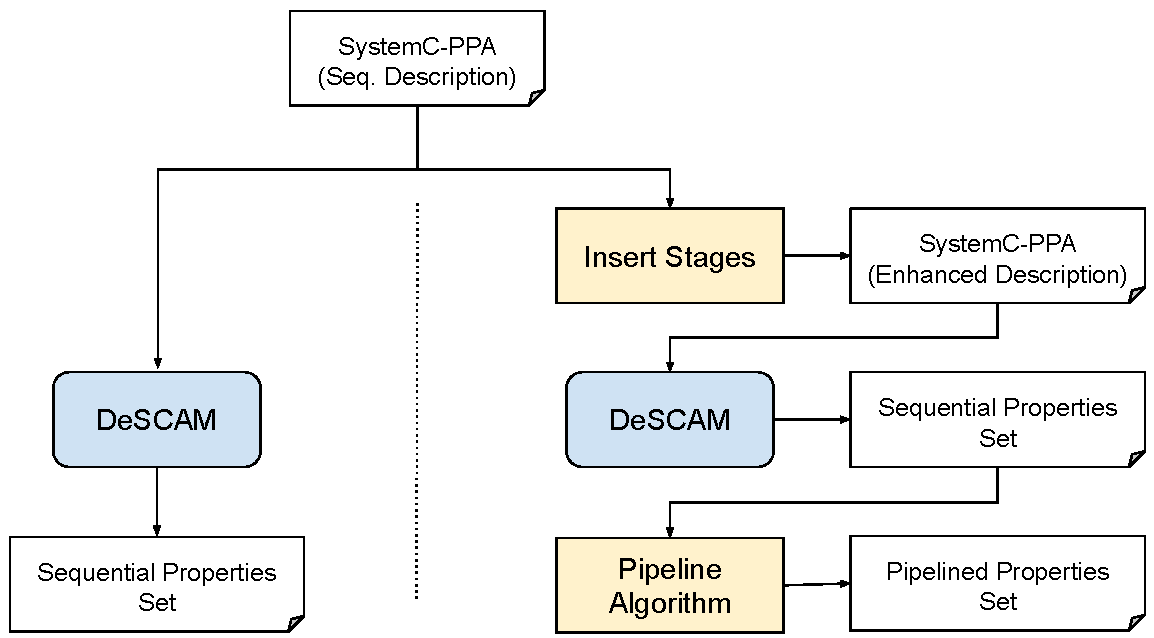
\includegraphics[width=0.85\textwidth]{images/new_pdd_flow.pdf}
	\caption{On the left, property generation with DeSCAM for the original PDD flow. On the right, extension of the PDD flow to better support of pipelined processors.}
	\label{fig:new-pdd-flow}
\end{figure}

In the same manner as the original flow, the extended PDD flow starts with a description at the architectural-level, which is PPA compliant. Before applying the description to DeSCAM, the SystemC-PPA model is modified to include information about the pipeline behaviour resulting in an enhanced PPA description. This description can be applied to DeSCAM which will generate a sequential property set of \textit{micro properties} (to be detailed later in this section). Finally, the \textit{Pipeline Algorithm} can merge the micro properties generating a property set with \textit{pipeline properties}.

The \textit{Insert Stages} phase allows the designer to include information about the desired pipeline structure into the SystemC-PPA model. It is important to emphasise that the designer does not have to translate the concurrent pipeline behaviour from the RTL implementation into the ESL model. The designer needs simply to include information about the desired pipeline stages at the appropriate points. This is done by calling the function \textit{insert\_state()} at the points in the data path of the ESL model corresponding to each pipeline stage. This function call will not influence the sequential behaviour of the simulation for the model at the system-level.

The \textit{insert\_state()} function is interpreted by the DeSCAM tool as a directive to include an important state in the PPA for that respective position in the code. Without this directive, the important states were only generated for communication calls, which affects the \textit{I/O} behaviour (see Sec.~\ref{subsection:PDD-flow}). Consider the regular PPA in Fig.~\ref{subfig:ppa-seq} extracted from a sequential ESL model without the manually inserted stages. If a call to insert a state for each pipeline stage is used, the resulting enriched PPA such the one in Fig.~\ref{subfig:ppa-pipe-processor} is obtained.

\begin{figure}[htb!]
\centering
\begin{subfigure}[b]{0.45\textwidth}
  \centering
	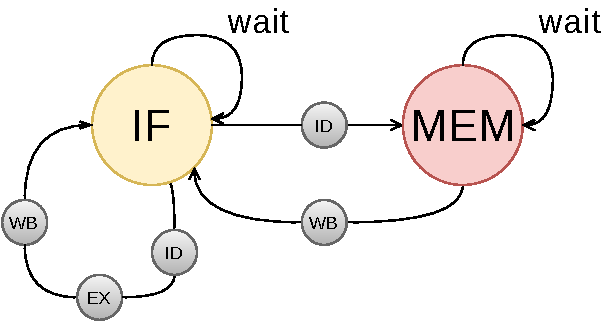
\includegraphics[width=0.9\textwidth]{images/PPA_old.pdf}
	\caption{PPA for regular PDD flow.}
	\label{subfig:ppa-seq}
\end{subfigure}
\hfill
\begin{subfigure}[b]{0.45\textwidth}
  \centering
	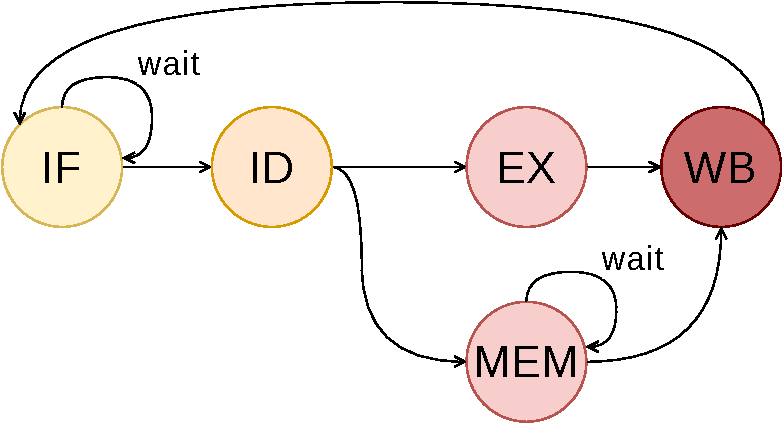
\includegraphics[width=0.9\textwidth]{images/PPA_new.pdf}
	\caption{PPA for extended PDD flow.}
	\label{subfig:ppa-pipe-processor}
\end{subfigure}
\caption{(a) PPA for a sequential SystemC-PPA processor description like in Fig.~\ref{fig:ppa-seq}. (b) Enriched PPA for an enhanced SystemC-PPA processor description with states inserted for each pipeline stage.}
\label{fig:ppa-old-and-new}
\end{figure}

The enriched PPA of Fig.~\ref{subfig:ppa-pipe-processor} derived from an enhanced SystemC-PPA has one important state for each pipeline stage. As a result, the property set generated by DeSCAM will also be different. Let us consider an \textit{ADD} instruction for a 4-stage pipeline processor as an example. The property generated by DeSCAM for a regular sequential SystemC-PPA description is seen in the listing of Fig.~\ref{fig:ex-pdd-add-ppt}. Since only one important state, for instance \textit{IF}, is present on the execution path of an \textit{ADD} instruction, only one property is generated for describing the behaviour of this instruction. This can be also seen on the PPA of Fig.~\ref{subfig:ppa-seq} where the \textit{ADD} operation corresponds to a single edge starting  and ending on important state \textit{IF}. On the other hand, an \textit{ADD} instruction execution on the enriched PPA of Fig.~\ref{subfig:ppa-pipe-processor} corresponds to four edges. Therefore, four properties will be generated for this single instruction. These operations describing the behaviour between two pipeline stages are named \textit{micro operations}, or \textit{micro properties}. The listing on Fig.~\ref{fig:add-if-id-micro-ppt} shows two examples of micro properties. The property in Fig.~\ref{subfig:add-if-micro-ppt} corresponds to the operation between the \textit{IF} and \textit{ID} stages, and the property in Fig.~\ref{subfig:add-id-micro-ppt} the operation when the IUV goes from stage \textit{ID} to \textit{EX}.

\begin{figure}[htb!]
     \centering
     \begin{subfigure}[b]{\textwidth}
         \begin{lstlisting}
    property PDD_ADD_IF;
    dependencies: no_reset;
    for timepoints:
        t_end = t+1;
    freeze:
        PC_at_t = PC@t;
    assume:
        at t: IF;
    prove:
        at t_end: ID;
        at t_end: PC == PC_at_t + 4;
        at t_end: fetched_instr == instr_in_sig;
        at t_end: operands == getOperandsFromRegFile(fetched_instr);
        during [t+1, t_end-1]: instr_req_out_notify == false;
        at t_end: instr_req_out_notify == true;
        during [t+1, t_end]: data_req_out_notify == false;
    end property;\end{lstlisting}
         \caption{Micro property describing operation from \textit{IF} stage to \textit{ID} stage.}
         \label{subfig:add-if-micro-ppt}
     \end{subfigure}
     \hfill
     \begin{subfigure}[b]{\textwidth}
         \begin{lstlisting}
    property PDD_ADD_ID;
    dependencies: no_reset;
    for timepoints:
        t_end = t+1;
    freeze:
        PC_at_t = PC@t,
        fetched_instr_at_t = fetched_instr@t;
    assume:
        at t: ID;
        at t: getInstrType(fetched_instr) == ADD;
    prove:
        at t_end: EX;
        at t_end: PC == PC_at_t;
        at t_end: fetched_instr == fetched_instr_at_t;
        at t_end: ex_regData == operands.rs1 + operands.rs2;
        at t_end: ex_regAddr == operands.rd;
        at t_end: ex_regWrEn == true;
        during [t+1, t_end]: instr_req_out_notify == false;
        during [t+1, t_end]: data_req_out_notify == false;
    end property;\end{lstlisting}
         \caption{Micro property describing operation from \textit{ID} stage to \textit{EX} stage.}
         \label{subfig:add-id-micro-ppt}
     \end{subfigure}
        \caption{Example of micro properties generated for an \textit{ADD} instruction from an enhanced SystemC-PPA processor description with states inserted to each pipeline stage. The property in (a) refers to the transition between \textit{IF} and \textit{ID} stages, and the property in (b) the transition between \textit{ID} and \textit{EX}.}
        \label{fig:add-if-id-micro-ppt}
\end{figure}

One problem with describing the behaviour of a single instruction with multiple micro properties is the loss of intuitiveness for the designer. It is more natural to describe an instruction behaviour spawning over all pipeline stages. A second problem is that each micro operation generated will describe the behaviour of all \textit{outputs} and visible registers. As discussed in Sec.~\ref{section:pdd-pipe-processor}, this makes the property set impossible to hold because each property, in this pipelined processor context, should prove only the values of interest for the corresponding stage. An example of this problem can be observed in the micro properties of Fig,~\ref{fig:add-if-id-micro-ppt}. The PC behaviour is correctly proven to be incremented in (a) when the IUV is on the \textit{ID} stage. However, in (b), the PC is proven to remain with the same value. This is not true as the PC is normally incremented in every clock cycle as a new instruction is fetched. Another inconsistency refers to the output signal requesting a new instruction, \textit{instr\_req\_out\_notify}. In the  commitments of (b), the signal is proven to be de-asserted, which is not the expected behaviour of a pipeline processor that requests a new instruction every clock cycle when there is no \textit{stall}.

The other additional phase included on the extended PDD flow of Fig.~\ref{fig:new-pdd-flow} is the Pipeline Algorithm. This proposed algorithm combines the micro properties referring to a single instruction into a pipeline property. This property describes the behaviour of the instruction executing throughout all pipeline stages, similarly to the property shown in the listing of Fig.~\ref{fig:ex-add-ppt}. The Pipeline Algorithm is detailed in Sec.~\ref{section:pipe-algorithm}.

The notion of completeness discussed in Sec.~\ref{section:ipc-pipe-processor} and Sec.~\ref{section:s2qed} still applies. The set of pipeline properties generated by the algorithm represents the set of constrained properties that considers the IUV executing in an empty pipeline. For passing the case-split test and achieving completeness, a set of \SSQED{} properties has to be proven.

Finally, in addition to the HDL template that can be generated by DeSCAM in order to assist the designer on the RTL implementation, see Sec.~\ref{subsection:PDD-flow}, a new plugin  for DeSCAM was developed in this work. This plugin can be optionally used by the designer to automatically generate a top design in HDL creating the environment to prove the \SSQED{} properties. The plugin is detailed in Sec.~\ref{section:plugio-s2qed-top}.

\section{Generating the Pipeline Properties}
\label{section:pipe-algorithm}

The Pipeline Algorithm proposed in this work converts a property set of micro operations into a set of pipeline properties. Given a processor description at the architectural-level including the information of each pipeline stage by state insertion, the DeSCAM tool will generate a sequence of properties for each instruction from the ISA of the processor model. The algorithm will merge the sequence of properties for each instruction into a single pipeline property. 

The listing in Fig.~\ref{fig:sysc-pipe-proc} shows an example of a SystemC-PPA compliant processor description. For simplicity, the presented ESL implementation omits some code such as variable declarations and function implementations. The purpose of this example is to illustrate one possible implementation of a 4-stages pipeline processor at the architectural-level that will be used throughout this section to help understanding the proposed algorithm.

\begin{figure}[htb!]
    \begin{lstlisting}[language=c++]
    class pipelined_processor : public sc_module {
        //ports for communication with instr mem
        master_in<unsigned int> instr_in;
        master_out<bool> instr_req_out;
        //ports for communication with data mem
        master_in<unsigned int> data_in;
        blocking_out<CUtoME_IF> data_req_out;
        void fsm() {
            nextsection = Sections::FETCH_PH;
            while (true){
                section = nextsection;
                if (section == Sections::FETCH_PH){
                    insert_state("IF");
                    instr_in->master_read(fetched_instr);
                    nextsection = Sections::DECODE_PH;
                } else if (section == Sections::DECODE_PH){
                    PC = PC + 4;
                    instr_req_out->master_write(PC);
                    operands = getOperFromRegFile(fetched_instr);
                    insert_state("ID");
                    nextsection = Sections::EXE_MEM_PH;
                } else if (section == Sections::EXE_MEM_PH) {
                    if (getInstrType(fetched_instr) == ADD) {
                        ex_regData = operands.rs1 + operands.rs2;
                        ex_regAddr = operands.rd;
                        ex_regWrEn = true;
                        insert_state("EX");
                    } else if (getInstrType(fetched_instr) == LOAD) {
                        ex_regAddr = operands.rd;
                        ex_regWrEn = true;
                        memAccess.addrIn = operands.rs1 + operands.imm; 
                        memAccess.wrEn = false;
                        data_req_out->write(memAccess, "MEM");
                        data_in->master_read(ex_regData);
                    } else {} //Other Instructions[...] 
                    nextsection = Sections::WRITEBACK_PH;
                } else if (section == Sections::WRITEBACK_PH) {
                    wb_regWrEn = ex_regWrEn;
                    wb_regAddr = ex_regAddr;
                    wb_regData = ex_regData;
                    insert_state("WB");
                    RegFile[wb_regAddr] = (wb_regWrEn) ? wb_regData : RegFile[wb_regAddr];
    }}}};\end{lstlisting}
    \caption{SystemC-PPA description of a 4-stage pipeline processor}
    \label{fig:sysc-pipe-proc}
\end{figure}

The \textit{pipelined\_processor} has two communication interfaces. One used to communicate with the instruction memory, and the other for data memory transactions. The instruction memory interface is of the type \textit{Master}, see Sec.~\ref{subsection:PPA}, and it has two signals. One \textit{output} for requesting a new instruction to a specific address, and an \textit{input} to read the instruction. The data memory interface also has two \textit{ports}. One \textit{blocking output} to send data request, and a \textit{Master input} to read the requested data from the memory.

The module has one main function called \textit{fsm()}, which runs infinitely and implements the behaviour of the processor. The variable \textit{section} keeps track of on which pipeline stage the current instruction is running. Starting from the \textit{FETCH\_PH} section, each instruction will execute in one pipeline stage at time. For each stage, the function \textit{insert\_state()} (lines 13, 20, 27 and 41) is called in order to create an \textit{important state} at the PPA extracted from this ESL model. Nonetheless, the simulation at the system-level is still sequential, and each instruction is only going to be executed after the previous one is finished.

The ESL model in the example depicts the behaviour of two instructions in specific: \textit{ADD} and \textit{LOAD}. The only implementation difference between them is at the \textit{EXE\_MEM\_PH} section, from line 23 to line 36. This section represents the \textit{EX} stage for the \textit{ADD} instruction, where a new state is inserted (line 27), and the computation of the addition operation with the respective operands is done (line 24). Observe that for the \textit{LOAD} instruction the manual insertion of a new state is not required because the data memory \textit{port} is of type \textit{blocking}. Therefore, this transaction demands a synchronization which is translated into a new important state when the PPA is generated. All the other sections are the same for both instructions. In the \textit{FETCH\_PH} phase, a new instruction is fetched from memory. In the \textit{DECODE\_PH} phase, the PC is incremented, and the \textit{opcode} and \textit{operands} are extracted from the fetched instruction. In the \textit{WRITE\_BACK\_PH} phase, the result from the ALU or the data fetched from the memory is written to the register file, line 42.

When this ESL model is parsed by DeSCAM, a set of properties that comprises the \textit{reset property}, the regular properties and the \textit{wait properties} is generated. For the \textit{ADD} instruction, four micro properties are generated corresponding to the transitions between the pipeline stages \textit{IF}, \textit{ID}, \textit{EX}, \textit{WB} and back to \textit{IF}, i.e. each operation corresponds to an edge in the PPA of Fig.~\ref{subfig:ppa-pipe-processor}. Two of these micro properties are already shown in Fig.~\ref{fig:add-if-id-micro-ppt}. The property in (a) for the transition from \textit{IF} to \textit{ID}, and the property in (b) for the transition between \textit{ID} and \textit{EX}. The other two micro properties generated for the \textit{ADD} instruction are presented in Fig.~\ref{fig:add-ex-wb-micro-ppt}. These micro properties correspond to the transition (a) from \textit{EX} to \textit{WB}  and (b) from \textit{WB} to \textit{IF}. 

\begin{figure}[htb!]
     \centering
     \begin{subfigure}[b]{\textwidth}
         \begin{lstlisting}
    property PDD_ADD_EX;
    dependencies: no_reset;
    for timepoints:
        t_end = t+1;
    freeze:
        PC_at_t = PC@t,
        fetched_instr_at_t = fetched_instr@t;
    assume:
        at t: EX;
    prove:
        at t_end: WB;
        at t_end: PC == PC_at_t;
        at t_end: fetched_instr == fetched_instr_at_t;
        at t_end: wb_regWrEn = ex_regWrEn;
        at t_end: wb_regAddr = ex_regAddr;
        at t_end: wb_regData = ex_regData;
        during [t+1, t_end]: instr_req_out_notify == false;
        during [t+1, t_end]: data_req_out_notify == false;
    end property;\end{lstlisting}
         \caption{Micro property describing operation from \textit{EX} stage to \textit{WB} stage.}
         \label{subfig:add-ex-micro-ppt}
     \end{subfigure}
     \hfill
     \begin{subfigure}[b]{\textwidth}
         \begin{lstlisting}
    property PDD_ADD_WB;
    dependencies: no_reset;
    for timepoints:
        t_end = t+1;
    freeze:
        PC_at_t = PC@t,
        fetched_instr_at_t = fetched_instr@t;
    assume:
        at t: WB;
    prove:
        at t_end: IF;
        at t_end: PC == PC_at_t;
        at t_end: fetched_instr == fetched_instr_at_t;
        at t_end: RegFile[wb_regAddr] == (wb_regWrEn) ? wb_regData : RegFile[wb_regAddr];
        during [t+1, t_end]: instr_req_out_notify == false;
        during [t+1, t_end]: data_req_out_notify == false;
    end property;\end{lstlisting}
         \caption{Micro property describing operation from \textit{WB} stage to \textit{IF} stage.}
         \label{subfig:add-wb-micro-ppt}
     \end{subfigure}
        \caption{Example of micro properties generated for an \textit{ADD} instruction from an enhanced SystemC-PPA processor description with states inserted to each pipeline stage. The property in (a) refers to the transition between \textit{EX} and \textit{WB} stages, and the property in (b) the transition between \textit{WB} and \textit{IF}. }
        \label{fig:add-ex-wb-micro-ppt}
\end{figure}

The Pipeline Algorithm will convert the micro properties set into a pipeline properties set that comprises the reset property, and merge the regular micro properties and wait properties into pipeline properties. The refinement of the reset property follows the regular property refinement of the PDD flow in \cite{paper-pdd}. Constraints can be added if needed, and $t\_end$ must be updated to the appropriate time point.

The algorithm to merge the regular micro properties and wait properties into a set of pipeline properties consists of three major steps:

\begin{enumerate}
\item \textit{Find the root state}: the \textit{root} state is the first important state to be reached by the system after \textit{reset}. This node within the PPA is used in step two as the start point for finding cycles;
\item \textit{Find cyclic paths}: In this step, all the cyclic sub-graphs of the PPA that start and end in the \textit{root} state are identified. For the PPA in Fig.~\ref{subfig:ppa-pipe-processor}, two cyclic paths are present, \textit{IF-ID-EX-WB-IF} and \textit{IF-ID-MEM-WB-IF}. The edges referring to the \textit{wait} operations are ignored in this step and converted into \textit{bounded wait for input} in step three.
\item \textit{Merging micro properties}: In this last step, the micro properties belonging to a cyclic path are converted into a single pipeline property. The algorithm to merge micro properties within the same cycle is detailed next. 
\end{enumerate}

\subsection*{The Merging Algorithm}

The procedure for merging a sequence of micro properties referring to the operations in a cyclic sub-graph of the PPA is presented in the flowchart in Fig.~\ref{fig:algorithm-flow}. The syntax employed for the algorithm corresponds to the proprietary language ITL \cite{onespin}, as this syntax is more intuitive and readable than e.g. SVA. Nonetheless, the procedure can be easily adapted to other verification languages. 

\begin{figure}[htb!]
	\centering
	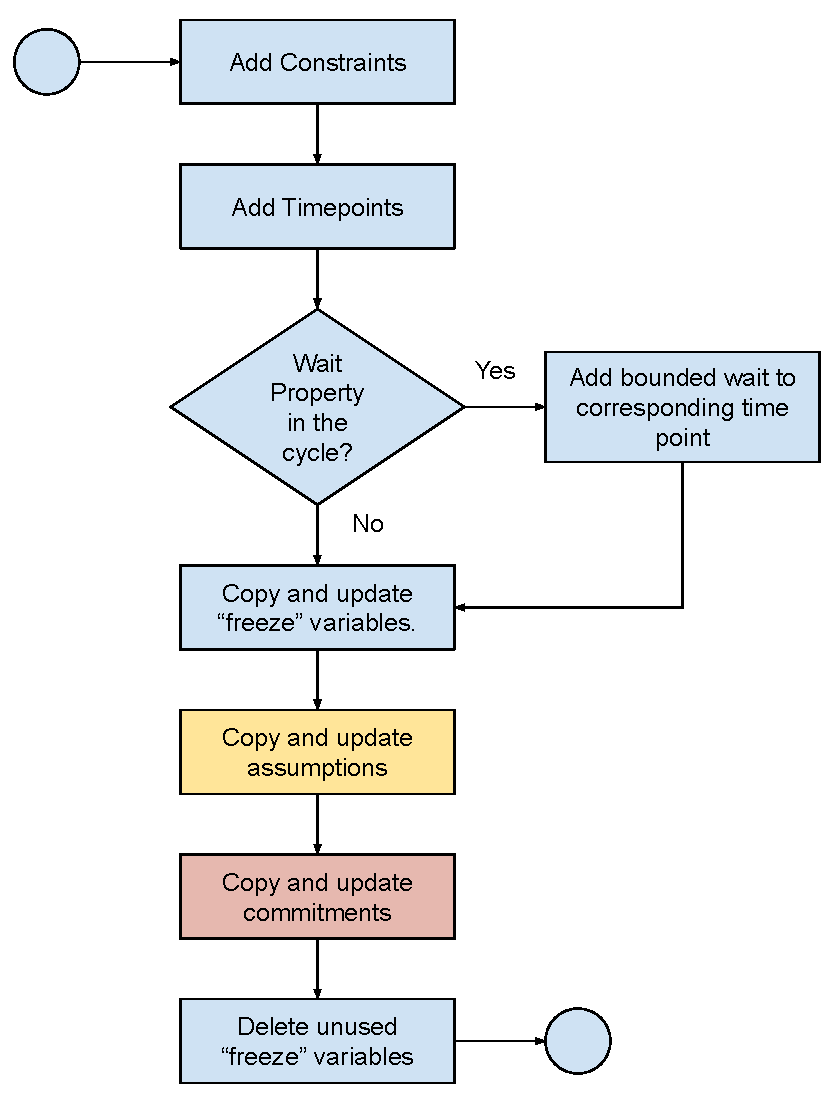
\includegraphics[width=0.7\textwidth]{images/algorithm.pdf}
	\caption{Flowchart for the merging algorithm that combines a sequence of micro properties of a cyclic sub-graph of the PPA into a Pipeline Property.}
	\label{fig:algorithm-flow}
\end{figure}

The first step of the merging algorithm is “Add Constraints”. As shown in the micro properties of Fig.~\ref{fig:add-ex-wb-micro-ppt}, DeSCAM generates the properties already including one constraint, \textit{no\_reset}. This constraint informs the \textit{property checking tool} that, for the duration of the operation, there should be no \textit{reset} signal. At this step, the designer must include any other constraints that are valid for the entire duration of the operation. One example is a constraint that specifies the memory protocol, so the tool knows how the memory \textit{input} signals behave.

For the “Add Timepoints” step, one timepoint variable is created referring to the commitments of each micro property. The micro properties include the $t\_end$ timepoint variable, see line 4 of Fig.~\ref{subfig:add-if-micro-ppt}, and these timepoints are integrated to the resulting pipeline property, e.g. $t\_id$, $t\_ex$, and $t\_wb$ representing the time for each pipeline stage.

Next, the cyclic path is analysed in order to identify if there are wait operations present. If that is the case, the step “Add bounded wait to corresponding timepoint” is executed, where each wait operation must be converted into a \textit{bounded wait} to the corresponding \textit{input} signal and included for the right timepoint. The micro properties in Fig.~\ref{fig:load-mem-wait-micro-ppt} show the transitions for a \textit{LOAD} instruction at the \textit{MEM} stage. In (a) the IUV is at stage \textit{MEM} and the \textit{sync} signal from the memory arrives. Then, the \textit{LOAD} instruction moves forward to the \textit{WB} stage. In (b), the wait operation proves that the IUV remains at the \textit{MEM} stage until the \textit{sync} signal comes. In this case, a \textit{bounded wait} for the \textit{input} signal \textit{data\_req\_out\_sync} is created at $t\_wb$, i.e. the timepoint corresponding to the write back stage.

\begin{figure}[htb!]
     \centering
     \begin{subfigure}[b]{\textwidth}
         \begin{lstlisting}
    property PDD_LOAD_MEM;
    dependencies: no_reset;
    for timepoints:
        t_end = t+1;
    freeze:
        PC_at_t = PC@t,
        fetched_instr_at_t = fetched_instr@t,
        data_in_sig_at_t = data_in_sig@t;
    assume:
        at t: MEM;
        at t: data_req_out_sync;
    prove:
        at t_end: WB;
        at t_end: PC == PC_at_t;
        at t_end: fetched_instr == fetched_instr_at_t;
        at t_end: wb_regWrEn = ex_regWrEn;
        at t_end: wb_regAddr = ex_regAddr;
        at t_end: wb_regData = data_in_sig_at_t;
        during [t+1, t_end]: instr_req_out_notify == false;
        during [t+1, t_end]: data_req_out_notify == false;
    end property;\end{lstlisting}
         \caption{Micro property describing operation from \textit{MEM} stage to \textit{WB} stage when the \textit{sync} signal from data memory arrives.}
         \label{subfig:load-mem-micro-ppt}
     \end{subfigure}
     \hfill
     \begin{subfigure}[b]{\textwidth}
         \begin{lstlisting}
    property PDD_LOAD_WAIT_MEM;
    dependencies: no_reset;
    for timepoints:
        t_end = t+1;
    freeze:
        PC_at_t = PC@t,
        fetched_instr_at_t = fetched_instr@t;
    assume:
        at t: MEM;
        at t: !data_req_out_sync;
    prove:
        at t+1: MEM;
        at t+1: PC == PC_at_t;
        at t+1: fetched_instr == fetched_instr_at_t;
        at t+1: instr_req_out_notify == false;
        at t+1: data_req_out_notify == false;
    end property;\end{lstlisting}
         \caption{Micro property describing the wait operation when the IUV is in the \textit{MEM} stage waiting for the synchronization signal from the data memory}
         \label{subfig:load-wait-micro-ppt}
     \end{subfigure}
        \caption{Example of micro properties generated for a \textit{LOAD} instruction from an enhanced SystemC-PPA processor description with states inserted to each pipeline stage. The property in (a) refers to the transition between \textit{MEM} and \textit{WB} stages, and the property in (b) shows the wait operation.}
        \label{fig:load-mem-wait-micro-ppt}
\end{figure}

In the “Copy and update ‘freeze’ variables step”, the variables present at the “\textit{freeze}” section of each micro property, e.g. line 6 of Fig.~\ref{subfig:add-if-micro-ppt}, are copied into the merged property. The names of the variables are updated to match the created timepoint for the corresponding micro operation.

The steps marked in yellow and red refer to merging assumptions and commitments. They are broken down into further steps and are presented in figures \ref{fig:algorithm-assumptions-flow} and \ref{fig:algorithm-commitments-flow}. The last step is to “Delete unused ‘freeze’ variables”, where the variables that are no longer used at the assumptions and commitments are excluded. 

\subsubsection*{Merging Assumptions}

\begin{figure}[htb!]
    \centering
	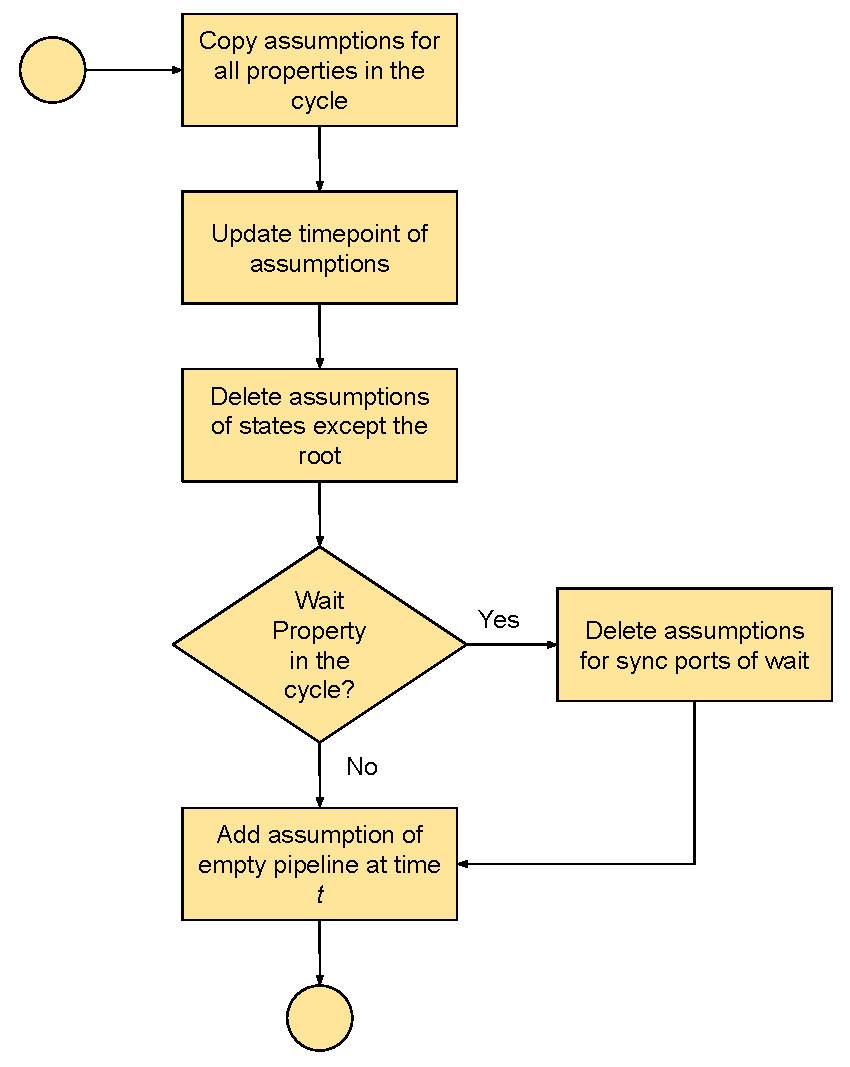
\includegraphics[width=0.7\textwidth]{images/algorithm_assumptions.pdf}
	\caption{Flowchart for merging assumptions from micro properties into assumptions of the pipeline property.}
	\label{fig:algorithm-assumptions-flow}
\end{figure}

The first step towards merging the assumptions, “Copy assumptions”, is shown in Fig.~\ref{fig:algorithm-assumptions-flow}, and it copies the assumptions for all micro properties in the cycle into the assumptions field of the pipeline property. Then, in the “Update timepoint of assumptions” step, the timepoints of assumptions are updated according to the timepoint created for the corresponding micro property. Next, it is the “Delete assumptions of states except the root” step. The resulting pipeline property will have its starting state at time $t$ being the \textit{root} state, e.g. the \textit{IF} state. The designer must refine this state to represent the \textit{ready to fetch} state reached after \textit{reset}.

If there is a wait operation in the cycle, the next step is “Delete assumptions for sync ports of wait” properties. This is necessary because the synchronization signal is already included at the \textit{bounded wait}.

The final step to complete the assumption part of the pipeline property is “Add assumption of empty pipeline at time $t$”. This assumption is not generated by DeSCAM and must be refined by the designer. It constrains the IUV to execute in an empty pipeline.

\subsubsection*{Merging Commitments}

\begin{figure}[htb!]
	\centering
	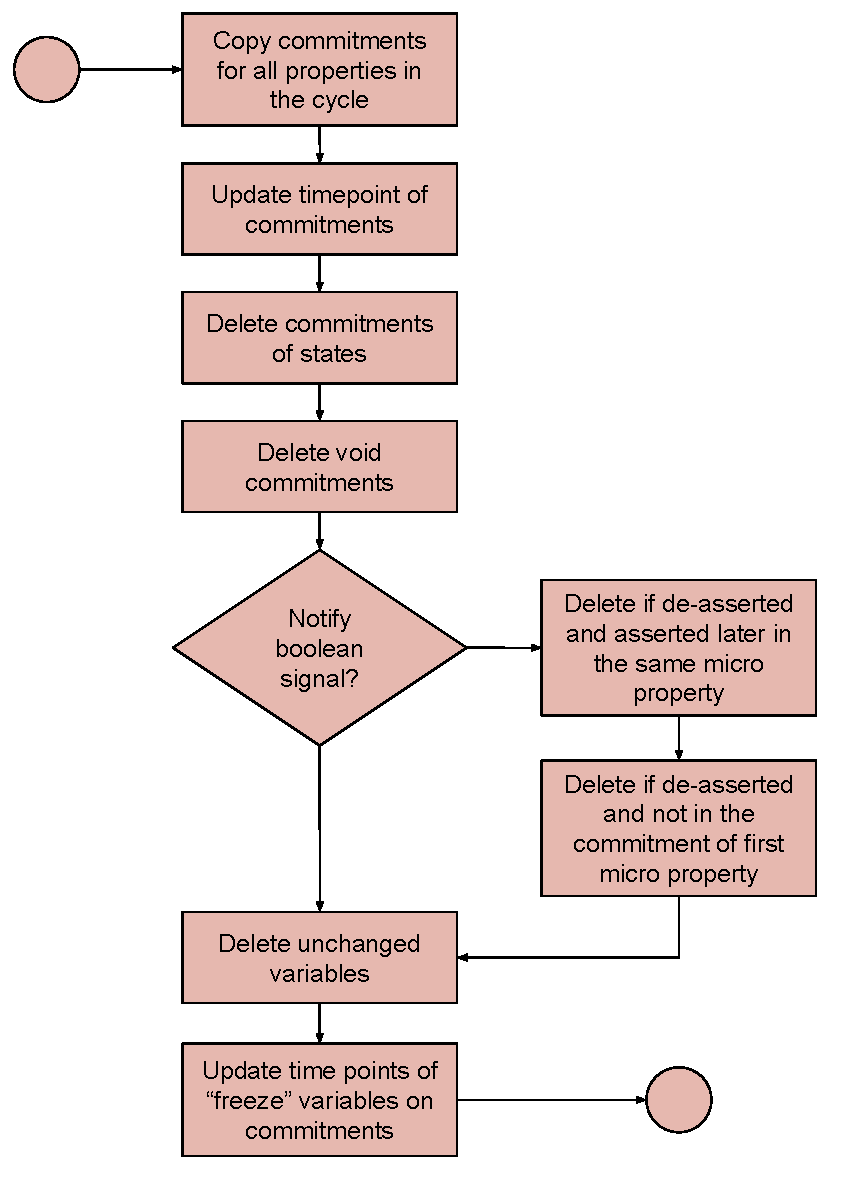
\includegraphics[width=0.7\textwidth]{images/algorithm_commitments.pdf}
	\caption{Flowchart for merging commitments from micro properties into commitments of the pipeline property.}
	\label{fig:algorithm-commitments-flow}
\end{figure}

Similarly to the assumptions, the commitment steps start with “Copy commitments for all properties in the cycle”, “Update timepoint of commitments”, and then “Delete commitments of states”. The next step is “Delete void commitments”, e.g. the commitment in line 14 of Fig.~\ref{subfig:add-id-micro-ppt}. This commitment selects a time interval between $t+1$ and $t\_end-1$, which is void. In practice, this commitment can be kept in the property as it will not interfere in the property checking. However, removing it increases the readability of the resulting property.

The next two steps are related to \textit{notify} signals derived from communication ports of the ESL model. The “Delete if de-asserted and asserted later in the same micro property” step is intended to delete the commitments where the \textit{notify} signals are de-asserted for a time interval and then asserted later in the same micro property. This is a consequence of the pipeline behaviour where the time of interest for the commitments of each micro operation is the timepoint of the current pipeline stage.

The “Delete if de-asserted and not in the commitment of first micro property” step refers to the refinement of the commitments that are not from the micro property starting from the \textit{root} state. The \textit{notify} signal is only kept if it is asserted, otherwise it is not important for that pipeline stage. Keeping such commitment would create contradictive commitments. This does not apply to the commitments from the first micro operation because any \textit{output} signal is determined at this time as a result of the empty pipeline assumption. The commitments in lines 18 and 19 of the property in Fig.~\ref{subfig:add-id-micro-ppt} are examples of commitments that are deleted by the merging algorithm.

The next step, “Delete unchanged variables”, follows the same idea and deletes the variables which values are assigned to the same previous value, e.g. commitments of lines 13 and 14 of Fig.~\ref{subfig:add-id-micro-ppt}.

“Update time points of ‘freeze’ variables on commitments” is the final step for refining the commitments. It changes the names of the “\textit{freeze}” variables according to the corresponding timepoint tag assigned to the referred micro property. E.g. the micro property in Fig.~\ref{subfig:add-id-micro-ppt} used the variable \textit{PC\_at\_t} in the commitment of line 13. Since the timepoint $t$ becomes $t\_id$ with the merging step, by this rule the variable would become $PC\_at\_t\_id$. 

One special case for this step refers to the signals derived from the data port of \textit{blocking} interfaces. Consider the commitment in line 18 of the property in Fig.~\ref{subfig:load-mem-micro-ppt}. The signal \textit{data\_in\_sig} corresponds to the message signal of the data memory \textit{blocking} port. This variable relates to the data that arrives with the \textit{sync} signal \textit{data\_req\_out\_sync} in the \textit{wait} operation. In this case, the variable in line 18 must be updated to the timepoint when the data comes after the wait, i.e. the timepoint with the \textit{bounded wait}, $t\_wb$.

\subsubsection*{Pipeline Properties}

The listing in Fig.~\ref{fig:add-ptt-merg-algorithm} shows a property resulting form the merging algorithm applied to the four micro properties, shown in Fig.~\ref{fig:add-if-id-micro-ppt} and Fig.~\ref{fig:add-ex-wb-micro-ppt}, generated for an \textit{ADD} instruction.

\begin{figure}[htb!]
    \begin{lstlisting}
    property PIPE_PDD_ADD;
    dependencies: 
        no_reset,
        instr_mem;
    for timepoints:
        t_id = t+1,
        t_ex = t_id+1,
        t_wb = t_ex+1,
        t_end = t_wb+1;
    freeze:
        PC_at_t = PC@t;
    assume:
        at t: IF;
        at t: empty_pipeline;
        at t_id: getInstrType(fetched_instr) == ADD;
    prove:
        at t_id: PC == PC_at_t + 4;
        at t_id: fetched_instr == instr_in_sig;
        at t_id: operands == getOperandsFromRegFile(fetched_instr);
        at t_id: instr_req_out_notify == true;
        during [t+1, t_id]: data_req_out_notify == false;
    
        at t_ex: ex_regData == operands.rs1 + operands.rs2;
        at t_ex: ex_regAddr == operands.rd;
        at t_ex: ex_regWrEn == true;
        during [t_id+1, t_ex]: data_req_out_notify == false;
    
        at t_wb: wb_regWrEn = ex_regWrEn;
        at t_wb: wb_regAddr = ex_regAddr;
        at t_wb: wb_regData = ex_regData;
        during [t_ex+1, t_wb]: data_req_out_notify == false;
    
        at t_end: RegFile[wb_regAddr] == (wb_regWrEn) ? wb_regData : RegFile[wb_regAddr];
        during [t_wb+1, t_end]: data_req_out_notify == false;
    end property;\end{lstlisting}
    \caption{Pipeline Property for an ADD instruction. This property is the result of the pipeline algorithm applied to the micro properties in Fig.~\ref{fig:add-if-id-micro-ppt} and Fig.~\ref{fig:add-ex-wb-micro-ppt}.}
    \label{fig:add-ptt-merg-algorithm}
\end{figure}

A constraint for the instruction memory protocol is added at the \textit{dependencies} part (line 4). One timepoint relating to the commitments of each micro property is added to the \textit{timepoints} part (lines from 6 to 9). The assumptions include the \textit{IF} state that must be refined into the \textit{ready to fetch} state, the \textit{empty\_pipeline} constraint, and the triggering condition at $t\_id$. This assumption determines the type of instruction, and it comes from the \textit{ID} micro property (Fig.~\ref{subfig:add-id-micro-ppt}). The commitments comprise four sets of commitments imported from each micro operation; the \textit{IF} operation from line 17 to 21, the \textit{ID} operation from line 23 to 26, the \textit{EX} operation from line 28 to 31, and the \textit{WB} operation in lines 33 and 34.

The listing in Fig.~\ref{fig:load-ptt-merg-algorithm} shows the timepoint part of a pipeline property for the \textit{LOAD} instruction. Line 6 shows the timepoint derived from the wait property where the \textit{bounded wait} upon the \textit{sync} signal is included. 

\begin{figure}[htb!]
    \begin{lstlisting}
    property PIPE_PDD_LOAD;
    [...]
    for timepoints:
        t_id = t+1,
        t_mem = t_id+1,
        t_wb = t_mem+1..max_wait_dmem waits_for (data_req_out_sync),
        t_end = t_wb+1;
    [...]
    end property;\end{lstlisting}
    \caption{Timepoint of a Pipeline Property for an \textit{LOAD} instruction.}
    \label{fig:load-ptt-merg-algorithm}
\end{figure}

After running the Pipeline Algorithm, a set of constrained pipeline properties is obtained. In order to have a complete set of properties, a set of \SSQED{} properties must be created as presented in Sec.~\ref{section:s2qed}. In order to further support the designer, a plugin for DeSCAM was implemented to create the setup environment to check the \SSQED{} property set. This implementation is presented in Sec.~\ref{section:plugio-s2qed-top}.

The extended PDD method for pipelined processors guides the hardware designer through simple steps when refining the generated property set. Nonetheless, it still constitutes more effort when compared to the original PDD method for non-pipelined designs. However, the majority of the steps composing the proposed algorithm can be automated and included as an extension for the DeSCAM tool. Future work will include both constrained pipeline properties set and \SSQED{} properties set as an extension to DeSCAM.

\section{The Plugin for the \SSQED{} Template}
\label{section:plugio-s2qed-top}

Sec.~\ref{section:s2qed} presents how the \SSQED{} approach can be employed to prove the case-split test and achieve completeness. In order to apply this approach, a special setup with two \textit{identical} and \textit{independent} instances of the DUV is required. A plugin for DeSCAM was implemented in this work in order to assist the hardware designer to create such setup. A schematic diagram of a configuration for allowing property check with the \SSQED{} approach is shown in Fig.~\ref{fig:s2qed-top-diagram}. 

\begin{figure}[htb!]
	\centering
	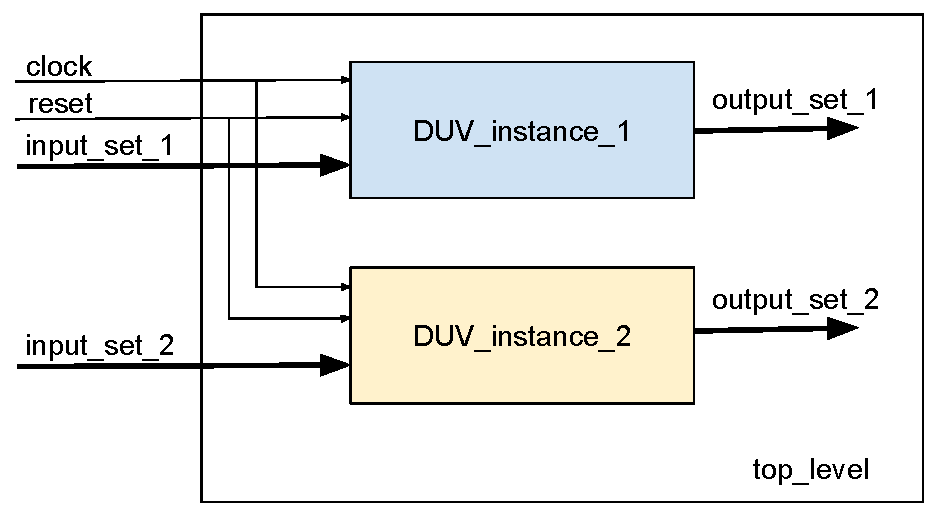
\includegraphics[width=0.7\textwidth]{images/top_s2qed.pdf}
	\caption{Diagram of a setup for proving the \SSQED{} model.}
	\label{fig:s2qed-top-diagram}
\end{figure}

The plugin can be optionally used by the designer to generate an HDL template for the configuration shown in Fig.~\ref{fig:s2qed-top-diagram}. The top-level generated has, besides the \textit{clock} and \textit{reset} signals, a duplicate set of \textit{inputs} matching the \textit{inputs} of the two DUV instances. The naming for \textit{inputs}, \textit{outputs} and signals corresponds to the names in the HDL template generated for the DUV by DeSCAM. During the \textit{refine-and-implement} process, the designer must update the top-level according to the changes made to the \textit{I/O ports} in the DUV. If the designer does not use the HDL template for the DUV, the structure of the top-level template for the \SSQED{} configuration can still be used. However, the \textit{I/O ports} and signals must be modified accordingly.

The listing in Fig.~\ref{fig:s2qed-top-example} shows an example of an HDL verification top-level generated for a DUV that has one \textit{input} vector of 32 bits and an \textit{output} signal. The ports of \textit{myDUV\_top} include \textit{input} signals for the two instances (lines 6 and 7). Port signals are created from line 10 to 14 for connecting the \textit{I/O} of both instances. The \textit{inputs} are assigned to their corresponding signals in lines 17 and 19.  Finally, the two DUV’s are instantiated from lines 21 to 33.

\begin{figure}[htb!]
    \begin{lstlisting}[language=c++]
    import top_level_types::*;
    import myduv_types::*;
    module myDUV_top (
        input logic clk,
        input logic rst,
        input bit[31:0] d_in_i1,
        input bit[31:0] d_in_i2
    );
    // Port signals for instance 1
    bit[31:0] d_in_s1;
    logic d_out_s1;
    // Port signals for instance 2
    bit[31:0] d_in_s2;
    logic d_out_s2;
    // Input signals assignments
    // Assignment fot instance_1
    assign d_in_s1 = d_in_i1;
    // Assignment fot instance_2
    assign d_in_s2 = d_in_i2;
    // Instance 1
    myDUV myDUV_inst_1 (
        .clk ( clk ),
        .rst ( rst ),
        .d_in ( d_in_s1 ),
        .d_out ( d_out_s1 )
    );
    // Instance 2
    myDUV myDUV_inst_2 (
        .clk ( clk ),
        .rst ( rst ),
        .d_in ( d_in_s2 ),
        .d_out ( d_out_s2 )
    );
    endmodule\end{lstlisting}
    \caption{Timepoint of a Pipeline Property for an \textit{LOAD} instruction.}
    \label{fig:s2qed-top-example}
\end{figure}

